%!TEX root =  ../Report.tex

\section{Current findings}
\label{sec:findings}

\subsection{PureCircuit and EndOfLine}
We will present several attempts and efforts we made across several problems and their
parsimonious reductions. First we want to introduce combine Kleene Logic with $\textbf{PPAD}$.
We define the following series of Problems


\begin{definitionbox}{Kleene Unary Numbers}{kleene-unary}
    \label{def:kleene-unary}
    Given a number $p \in M$, its unary representation can be depicted as a binary number $\{0,1\}^M$ such that: $k \in M \to 1^k \in \bar{M}$.
    Under Kleene algebra, we mainly refer to notations $M_k^n$ where $k,n,M \in \mathbb{N}_0$  such that:
    $$
        M^k_n \triangleq \{1^j\bot^k \mid \forall j \in \mathbb{N}_0 : j + k \leq n\}
    $$
\end{definitionbox}



\begin{definitionbox}{\scn{HF-StrongSperner} problem}{hf-strong-sperner}
    \textbf{Input}: A hazard-free circuit $\lambda: [M]^n \to \{-1, +1\}^n$, where $M \in n^{O(1)}$, that describes a \textit{StrongSperner} labelling,
    as explained in \ref{def:strong-sperner}, where the inputs are represented using Kleene Unary numbers \ref{def:kleene-unary}
    and $\#1(p) = \bar{p}$.\\
    \textbf{Output}: A point $p \in \bigtimes_{i \in [n]} M^1_n \cup M^0_n$ if and only if: $\lambda(p) =  \bot^n$.
\end{definitionbox}

We will mainly refer to a specific subset of these problems, which we will refer to as \scn{HF-DiscreteStrongSperner}.
The general idea is that we exploit the hazard-free property of the Strong Sperner function
In the original problem, we request for $d+1$ points as a solution to the problem. Due
to the assumption that $\forall p, p' \in S: \|p-p'\|_{\infty} \leq 1$, we can assume
they are all part of some high-dimensional cube. We abuse this notation by making the observation
that given $p \in [M^1]^n$, all the resolutions of $p$, resolve in a hypercube, as seen in the figure
one can observe that, we only need two points to create a panchromatic solution, where $\lambda(p) = \overline{\lambda(p')}$. These can create a lot of duplicate
solutions and therefore can behave unpredictably. We will mainly focus on subproblems of the \scn{HF-StrongSperner} where two cubes do not overlap.
More formally we define


\begin{figure}[h!]
    \centering
    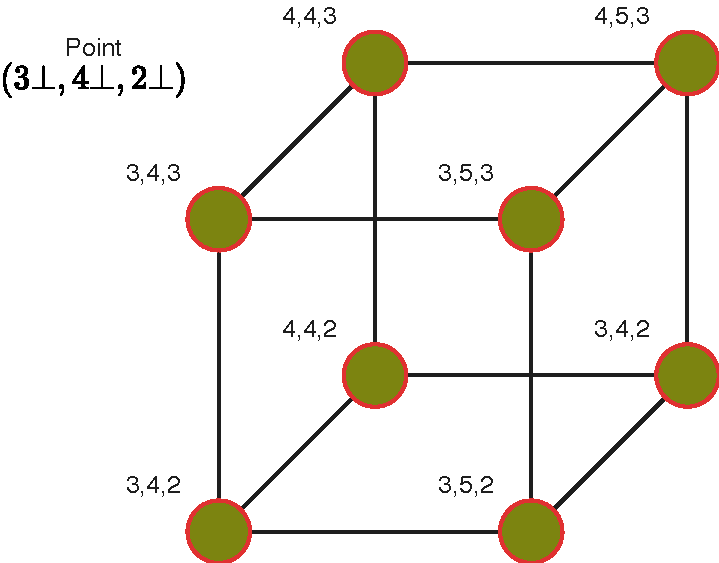
\includegraphics[width=0.3\textwidth]{Chapter3/1753903956-dissertation-drawing-assets.pdf}
    \caption{}
    \label{fig:chap-3:res-hyper}
\end{figure}


\begin{definitionbox}{\scn{HF-DiscreteStrongSperner} problem}{hf-strong-sperner}
    An \scn{HF-StrongSperner} instance $\lambda$ such that $\forall p \in [M^1]^n$, if $\lambda(p)= \bot^n$, then
    \begin{gather*}
        \forall j,i \in [n], [\phi^b_i(x)]_j \triangleq \begin{cases}
            x_i & \text{if }i \neq j \\
            b   & \text{if }i = j    \\
        \end{cases}\\
        \forall i \in [n],b \in\{0,1\},\exists j \in [n]: \forall x, x' \in \textbf{Res}(\phi^b_i(x)): [\lambda(x)]_j = [\lambda(x')]_j
    \end{gather*}
\end{definitionbox}

Lastly we introduce a specific subset of the above solutions where introduce antipodal panchromatic cubes.
In the specific type of solution said we argue that two opposite corners of a cube contain opposite colourings.
This notion of antipodal cubes is used in the majority of reductions across literature. More formally we say


\begin{definitionbox}{\textbf{MinRes} min and max resolution functions}{min-res-func}
    We use the \textbf{MinRes}, to denote the smallest resolution of a kleene string. More formally we can use the following equivalent definitions:
    \begin{align*}
        \forall x \in \{0,1,\bot\}^*, j \in [|x|]:  [\textbf{MinRes}(x)]_j
         & \triangleq \begin{cases}
                          x_i & \text{if } x_i \in \{0,1\} \\
                          0   & \text{otherwise}
                      \end{cases}
    \end{align*}
    For the maximum resolution we will use the $\textbf{MaxRes}$ function where we instead replace all $\bot$ with $1$ instead.
\end{definitionbox}

\begin{definitionbox}{\scn{HF-AntipodalStrongSperner} problem}{hf-strong-sperner}
    An \scn{HF-DiscreteStrongSperner} instance $\lambda$ such that $\forall p \in [M^1]^n$, if $\lambda(p)= \bot^n$,
    and denote $\textbf{MinRes}(x) = \hat{x}$ as the \textit{anchor} of the cube, then:
    $$
        \forall b \in \{0,1\}^n, j \in [n]: [\lambda(x + b)]_j = -[\lambda(x + 1^n \oplus b)]_j
    $$
\end{definitionbox}


\begin{claimbox}{Antipodal discrete squares}{antipodal-discrete-square}
    Given a panchromatic solution of a \scn{HF-AntipodalStrongSperner} $p$, it must be the case then that:
    $$
        \forall j \in \{-1, 1\}^n, \exists! x \in \textbf{Res}(p): \lambda(x) =  j
    $$
\end{claimbox}

\begin{proof}
    We proof by induction on $n$. Lets assume base case $n = 2$. We can observe that the only satisfying
    cube that is both antipodal and discrete, is some rotation of the following matrix
    $$
        \begin{pmatrix}
            \mp & +   \\
            -   & \pm \\
        \end{pmatrix}
    $$
    Where we denote $+ = (+, +), -=(-,-), \pm = (+,-)$ and $\mp = (-,+)$, we can observe indeed that the panchromatic square contains all the colourings.
    For the induction step, we can observe that if we want our colouring function to be both discrete and antipodal, then the following must suffice:
    given $k, k'$ the two resolutions of dimension $k+1$, we know that $[\lambda(p_{-(n+1)}(k))] = (b, \bot^n)$ for some $b \in \{0,1\}^n$. But that implies
    $[\lambda(p_{-(n+1)}(k'))] = (\bar{b}, \bot^n)$, which indicates a discrete antipodal panchromatic solution. Moreover if $p_{-(n+1)}$ cover $2^n$ labels,
    then the whole cube covers all $2^{n+1}$ labels, which by pigeonhole principle means that we must cover all possible combinations of colourings.
\end{proof}

All the problems above are clearly in \textbf{PPAD} as all of them reduce to the \textit{StrongSperner} problem, under only
binary inputs, since we make the assumption that all such circuits are inherently \textit{natural}. For the purposes of our current
research, we demonstrate a parsimonious reduction from \scn{HF-DiscreteStrongSperner} to \scn{PureCircuit}.


\begin{theorembox}{}{hf-discrete-to-pure}
    $$
        \textbf{\#PPAD}(\scn{HF-DiscreteStrongSperner}) \subseteq \textbf{\#PPAD}(\scn{PureCircuit})
    $$
\end{theorembox}

\begin{proof}
    Given an input instance $\Lambda$ of a \scn{HF-DiscreteStrongSperner}, we create a \scn{PureCircuit}
    \textit{Input nodes}, \textit{Output nodes}, \textit{Bit generator gadget} and \textit{Circuit application gadget}. To visualise our
    construction we will refer to the figure in \ref{fig:chap-3:pure-circuit}. Each of these parts describe the following:
    \begin{enumerate}
        \item  \textbf{Input nodes}: Vector of $n$ value nodes. Will be represented as $(x_i)_{i \in [n]} \in \mathbb{T}^n$.
        \item  \textbf{Bit generator gadget}: Given a value node $x_i$, apply the \textit{Bit generator} gadget such that we
              create Kleene unary number as defined in \ref{def:kleene-unary}, where $x^i \in M^{\leq 1}_n$. We will refer
              to the bit generator circuit as $C_i$.
        \item  \textbf{Circuit application gadget}: Since the above numbers form coordinates in a
              $[M]_0^n$ space, we apply the $\Lambda$ function to extract a set of output nodes $(u^i)_{i \in [n]} \in \gls{kleene-set}^n$.
        \item  \textbf{Output nodes}: We use the \texttt{Copy} gate to copy $u^i \to x_i$, for all $i \in [n]$.
    \end{enumerate}
    The 1st and last part of our construction is self-explanatory, we will analyse the other two sections in greater depth
    and prove some claims.

    \begin{figure}[h!]
        \centering
        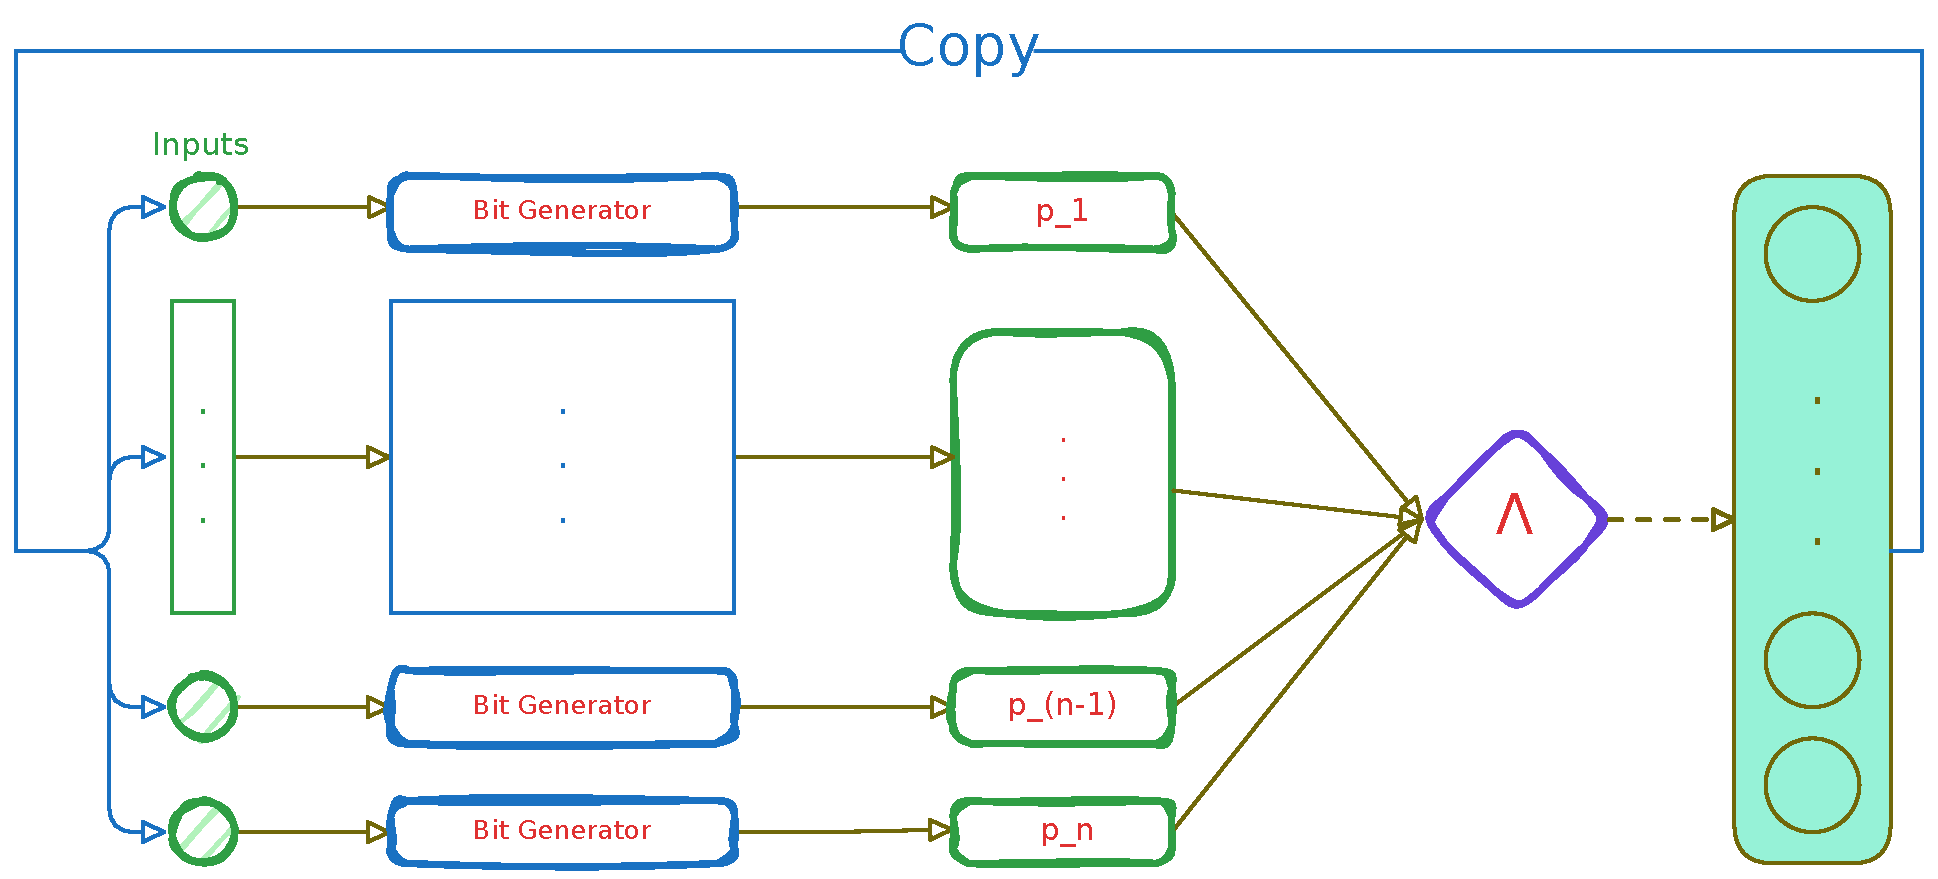
\includegraphics[width=0.5\textwidth]{Chapter3/pure-circuit-reduction.pdf}
        \caption{Pure Circuit construction visualisation}
        \label{fig:chap-3:pure-circuit}
    \end{figure}
    %% TODO reword 
    \paragraph*{Bit generator gadget} In order to create Kleene unary numbers we make use of a binary tree of \texttt{Purify} gates
    as seen in the figure \ref{fig:chap-3:purification-gadget}. We now claim that the current construction has certain desirable properties.


    \begin{figure}[h!]
        \centering %% TODO check the ordering of the graph
        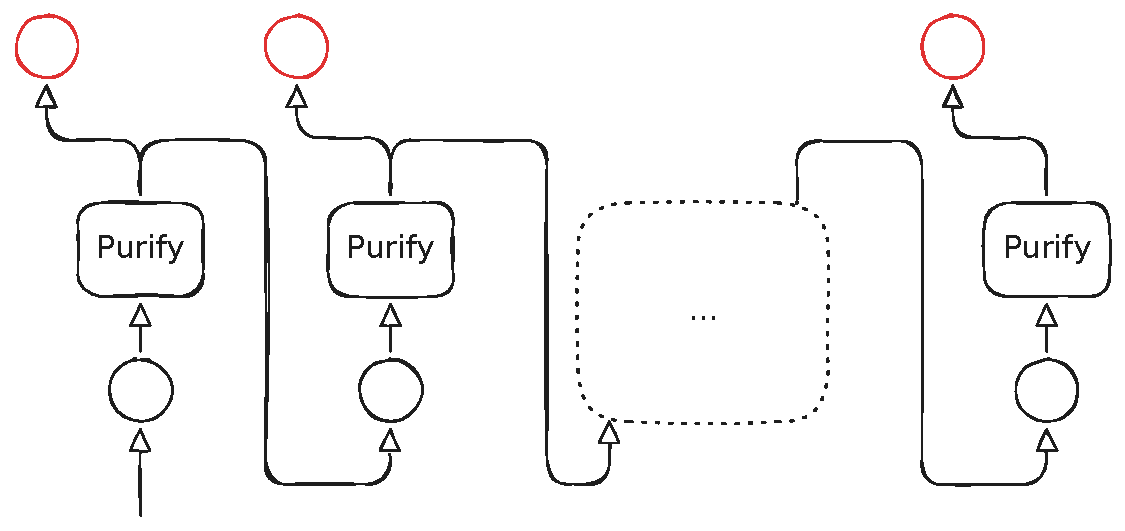
\includegraphics[width=0.5\textwidth]{Chapter3/purification-stage-construction.pdf}
        \caption{Purification gadget. The red nodes denote the outputs of the purification gadget.}
        \label{fig:chap-3:purification-gadget}
    \end{figure}

    \begin{claimbox}{Purification Claim}{chap-3:pur-claim}
        \label{clm:chap-3:pur-claim}
        Given the description of the bit generator gadget, we make the following two claims:
        \begin{enumerate}
            \item $b \in \{0,1\}^n: C_i(b) = b^n$
            \item $C_i(\bot) \in M^{\leq 1}_n$
        \end{enumerate}
    \end{claimbox}
    \begin{proof}
        From the definition of the \texttt{Purify} gate we know that
        $\forall b \in \{0,1\}: \texttt{Purify}(b) = (b,b)$, and therefore any subtree that takes a pure input, will copy its value
        to all its leafs, which follows our first claim directly. To the second part of our lemma, we can observe that
        the only valid outputs are $(0, \bot), (\bot,1), (0,1)$. Based on our previous observation, if a purify gate outputs
        a $(0, \bot)$ value, it will propagate $\bot$ to the rest of the tree and return $0$ in the current level,
        if the value is $(\bot/0, 1)$, the tree will return $\bot/0$ at the specific level, and then propagate $1$ to the rest of the leaves.
        This shows that all possible strings generated are of the form $1^k\bot^{0 \mid 1}0^{*}$.
    \end{proof}


    \paragraph*{Correctness and parsimonious argument}
    One can observe that the current construction is a valid construction, as we satisfy the arities of all gates and ensured
    that every node has an in-degree of $1$. We now make the following lemma

    \begin{lemmabox}{Correctness Lemma}{pure-correct-lem}
        A correct assignment corresponds to panchromatic cube in the original problem instance.
    \end{lemmabox}

    It suffices to show that every vector $x^i \in M^1_\bot$ and $\forall i \in [n]: \mathbf{x}[u^i] = \bot$.
    Assume that we have a correct assignment, and WLOG $\mathbf{x}[u^i] = 0$  for some $i \in [n]$.
    By our copy that, we know that $\mathbf{x}[u^i]= \mathbf{x}[x_i]$.
    By our  purification lemma {..} we know that $\mathbf{x}[x^i] = 0^i$.
    Since our circuit is hazard-free and applies the boundary conditions of the sperner problem, we know that
    $[\Lambda(x_{-i}(0))]_i = 1\neq \mathbf{x}[u^i]$. We can make a similar argument for $\mathbf{x}[u^i] = 1$.
    Therefore, a satisfying assignment corresponds to some panchromatic solution. Given that
    our instance is in \scn{HF-DiscreteStrongSperner}, it has to be the case that
    all $x_i \in M^1_n$, otherwise that would imply that there exists a $(n-1)$-subspace that also covers all the labels.
    This also shows that there exists a 1-to-1 mapping between a panchromatic cube and a satisfying assignment.
\end{proof}

Although the above reduction also works for the general $\textbf{HF-StrongSperner}$, the reduction is not parsimonious since
the PureCircuit will accept cubes in $(n-1)$ or lower subspaces.

\subsection{From the EndOfLine}
Although we have not managed to create a full reduction from the
\textit{EndOfLine} to \textit{PureCircuit}, we will demonstrate the closest
to what we can hope. First we acknowledge will mainly focus on
the \textit{RLeafD} problem, as it has been shown to be parsimonious to the \textit{EndOfLine} problem.
Chen et al. \cite{chen_Complexity2DDiscrete_2009}, has showed how to convert the problem from a graph
problem to a sperner problem but with linear colouring. We will first demonstrate how to do this with
bipolar instead. We will demonstrate how to apply the snake embedding technique to go reduce
the problem to an \textit{AntipodalStrongSperner} instance.

\paragraph*{Bipolar colouring of \textit{RLeafD}}

\begin{proof}
    We construct the same reduction as in the \textit{RLeafD} but with slight differences:
    We will use points $\mathbf{u}, \mathbf{v}, \mathbf{w} \in V_{2^k}$ and $\mathbf{p},\mathbf{q}, \mathbf{r} \in B_{2^{2k+5}}$ where
    $$
        B_n \triangleq \big\{  \mathbf{p} \in [n]^2 \big\}
    $$
    Moreover a polychromatic square will be denoted if all the points in the neighbouring squares satisfy the bipolar colouring.
    Morevoer below we will denote our colouring scheme for clarity:
    \begin{align*}
        +   & = (+1, +1) \\
        \pm & = (+1, -1) \\
        \mp & = (-1, +1) \\
        -   & = (-1, -1) \\
    \end{align*}


    First, we define mapping $\mathcal{F}: V_{2^k} \to B_{2^{2k+5}}$ such that
    $$
        \mathcal{F}(\mathbf{u}) = \begin{pmatrix}
            6 \mathbf{u}_{1} + 6 \\
            6 \mathbf{u}_{2} + 6 \\
        \end{pmatrix} \in B_{2^{2k+5}}
    $$
    Since $G \in C_{2^k}$, its edge-set can be decomposed into a collection of paths and cycles $(P_{i})_{i \in [m]}$.
    By using $\mathcal{F}$, every $P_{i}$ is mapped to a set $I(P_{i}) \subset B_{2^{2k+5}}$
    We will colour every point  on $I(P_{i})$ with $+$
    \begin{gather}
        P = \mathbf{u}^1,\dots,\mathbf{u}^t \text{, if P is a cycle } \mathbf{u}^1 = \mathbf{u}^t \\
        I(P) \triangleq \bigcup_{i \in [t-1]} I(u^tu^{t-1})
    \end{gather}
    A lot of \textit{Line reductions} under colouring use the notion of shielding. %% TODO add references to all problems
    Essentially we embed our lines and cycles in a grid, everything not a line is denoted as a negative charge $-$.
    All lines are denoted as positive charge $+$. To protect our lines from creating solutions, we cover them
    with $\pm, \mp$ lines. A visualisation can be seen in figure \ref{fig:chap-3:eol-shielding}.
    We define the following set to denote the set of shielding points around our paths.

    $$
        O(P) = \{  \mathbf{p} \in B_{2^{2k+5}} \setminus I(P) :\mid: \exists \mathbf{p}' \in I(P), \|p- p'\|_{\infty} = 1 \}
    $$

    \begin{figure*}
        \centering
        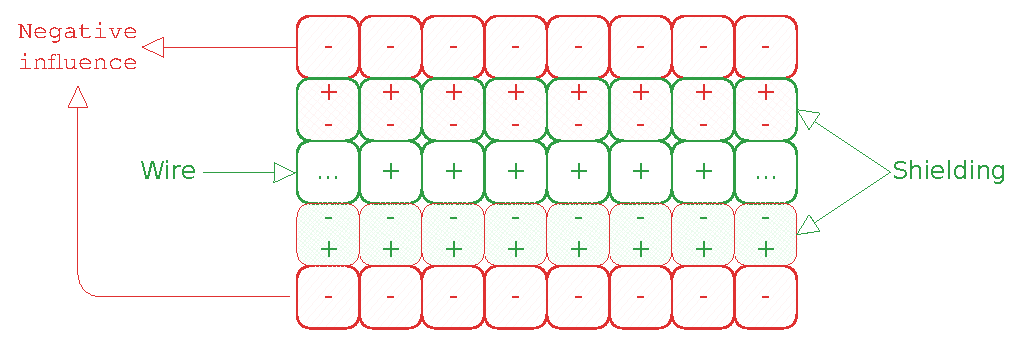
\includegraphics[width=0.5\textwidth]{Chapter3/coiling-eol.pdf}
        \caption{Shielding method on 2D-EoL embeddings.}
        \label{fig:chap-3:eol-shielding}
    \end{figure*}
    If $P$ is a simple path we can decompose $\{ \mathbf{s}_{p}, \mathbf{e}_{p} \} \cup L(P) \cup R(P)$ such that:
    $\mathbf{s}_{p} = \mathcal{F}(\mathbf{u}^1) + \Delta + \Delta^T$, where $\Delta = (\mathbf{u^1}- \mathbf{u}^2)$
    $\mathbf{e}_{p} = \mathcal{F}(\mathbf{u}^1) + \bar{\Delta} + \bar{{\Delta}}^T$, where $\bar{\Delta}= (\mathbf{u}^t - \mathbf{u}^{t-1})$
    Starting from $\mathbf{s}_{p}$,
    enumerate vertices in $O(P)$ clockwise as $\mathbf{s}_{p},\mathbf{q}^1,\dots,\mathbf{q}^{n_{1}}, \mathbf{e}_{p}, \mathbf{r}^1,\dots,\mathbf{r}^{n_{2}}$ such that
    \begin{align*}
        L(P) & = \{ \mathbf{q}^i \}_{i \in [n_{1}]}\ , \\
        R(P) & = \{ \mathbf{r}^i \}_{i \in [n_{2}]}\,  \\
    \end{align*}
    If $P$ is a simple cycle, then can can decompose $L(P) \cup R(P)$, where $L(P)$ contains all the vertices on the left side of the cycle and $R(P)$ all the vertices on the right side
    If $G$ is specified by $(K, 0^k) \subset C_{2^k}$, we can uniquely decompose the edge set into $P_{1}, \dots P_{m}$
    Every path is either a maximal path, or a cycle in $G$
    We can prove the following:
    \begin{lemmabox}{Disjoint Lemma}{lem:disj-lem}
        $$
            \forall i ,j : 1\leq i\neq j \leq m : \Big(I(P_{i}) \cup O(P_{i})\Big) \cap \Big( I(P_{j}) \cap O(P_{j}) \Big) = \emptyset
        $$
    \end{lemmabox}
    \begin{proof}
        %% TODO
    \end{proof}

    We can use the following to describe our colouring algorithm:

    \begin{algorithm}
        \caption{Turing machine $F$ with input $(p_1, p_2) \in B_{2^{2k+5}}$}
        \begin{algorithmic}
            % \If{$p_1 = 0$}
            %     \If{$p_2 \leq 6$}
            %         \Return $+$
            %     \Else
            %         \Return $\pm$
            %     \EndIf
            % \Elsif{$p_1 < 6$}
            %     \If{$p_2 = 6$}
            %         \Return $+$
            %     \Elsif{$p_2 < 6$}
            %         \Return $\mp$
            %     \Elsif{$p_2 = 7$}
            %         \Return $\pm$
            %     \Else
            %         \Return $-$
            %     \EndIf
            % \EndIf
            % \Return $M_K(\mathbf{p})$
            \If{$p_1 = 0$}
            \If{$p_2 \leq 6$}
            \State \Return $+$
            \Else
            \State \Return $\pm$
            \EndIf
            \ElsIf{$p_1 < 6$}
            \If{$p_2 = 6$}
            \State \Return $+$
            \ElsIf{$p_2 < 6$}
            \State \Return $\mp$
            \ElsIf{$p_2 = 7$}
            \State \Return $\pm$
            \Else
            \State \Return $-$
            \EndIf
            \Else
            \State \Return $M_K(\mathbf{p})$
            \EndIf
        \end{algorithmic}
    \end{algorithm}

    Where $M_{k}(\mathbf{p})$ is can be described with the following description:
    $$
        M_{k}(\mathbf{p})  =\begin{cases}
            +   & \text{ if } \exists i, \mathbf{p} \in I(P_{i})                \\
            \pm & \text{ if }\exists i, \mathbf{p} \in L(P_{i}) \vee p_{1} = 0  \\
            \mp & \text{ if } \exists i, \mathbf{p} \in R(P_{i}) \vee p_{2} = 0 \\
            -   & \text{ otherwise}
        \end{cases}
    $$
    We will call the path of nodes $(0,0) \to (0,6) \to(6,6)$ as the tail.
    An example of how such reduction looks like can be seen in figure \ref{fig:chap-3:eol-sperner-colouring}.
    \begin{figure}[h!]
        \centering
        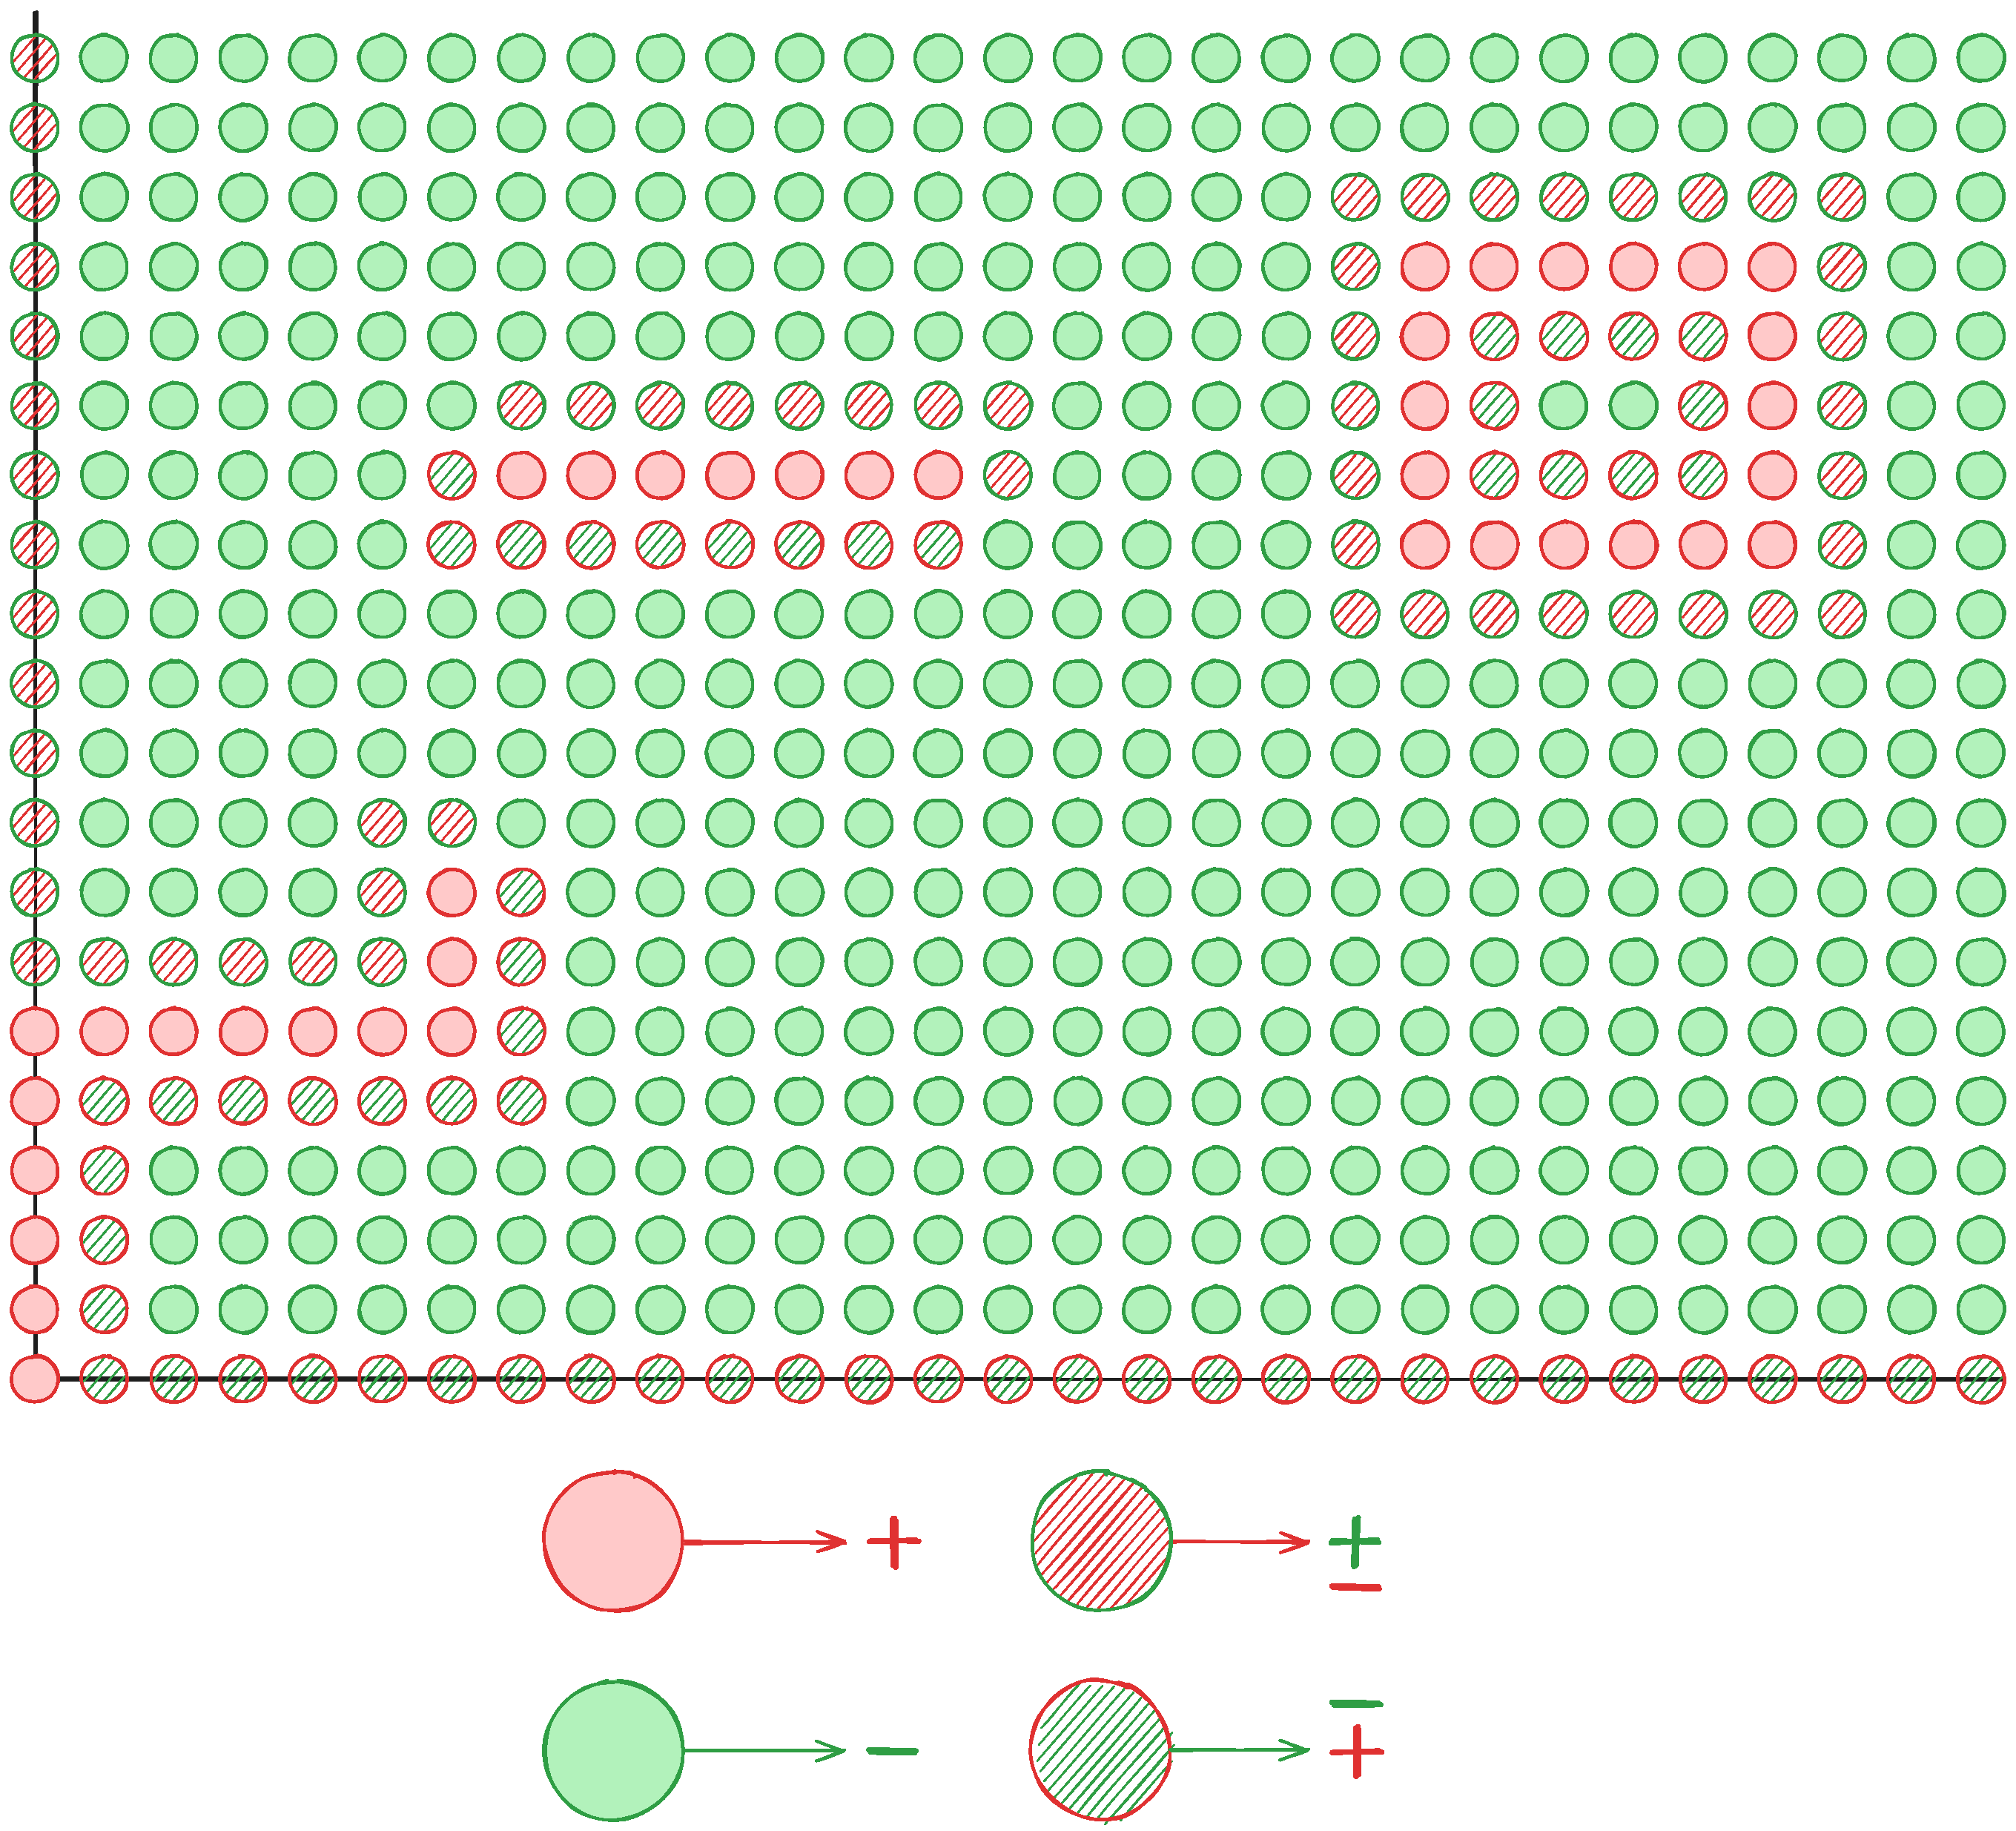
\includegraphics[width=0.5\textwidth]{Chapter3/2d-sperner-eol.pdf}
        \caption{2D EndOfLine Bipolar Colouring}
        \label{fig:chap-3:eol-sperner-colouring}
    \end{figure}


    \begin{lemmabox}{Correctness Lemma}{2d-eol-corr-lemma}
        The following statements hold correct:
        \begin{enumerate}
            \item $\forall i,j: \min_{x \in P_{i}, y\in P_{j}} \|\mathcal{F}(x) - \mathcal{F}(y) \|_{\infty} > 4$
            \item All polychromatic squares represent solutions
        \end{enumerate}
    \end{lemmabox}

    To prove the first statement, assume we have  $a,b \in V_{2^k}: \|a - b\|_{\infty} > 1$. WLOG assume
    $a -b = (x,y)$ for some $x,y \in \mathbb{N}$ which implies the following:
    \begin{gather*}
        \mathcal{F}(a) = \mathcal{F}\begin{pmatrix}
            b_{x} + x \\
            b_{y} + y \\
        \end{pmatrix} = \begin{pmatrix}
            6b_{x}+6x + 6 \\
            6b_{x}+6y + 6 \\
        \end{pmatrix} \\ \\
        \mathcal{F}(a) - \mathcal{F}(b) =  \begin{pmatrix}
            6x \\
            6y \\
        \end{pmatrix}
    \end{gather*}

    Since $x + y > 0 \implies \|\mathcal{F}(a) - \mathcal{F}(b)\|_{\infty} \geq 6 > 4$.  This statement is meant space all lines far enough such that the colouring
    of each one won't affect the other.

    To show our second part of our solution, we can observe that:
    All nodes that are not boundary nor not in $\bigcup_{i }I(P_{i}) \cup L(P_{i}) \cup S(P_{i})$ are coloured $-$.
    All $+$ coloured nodes are on the tail and in the line, all non-tail nodes are cushioned by $\pm, \mp$ and every non-tail node is not poly chromatic.
    All $-$ elements do not affect $\pm,\mp$  coloured nodes.
    Since all lines are sufficiently apart from each other, it suffices to check only the ends of paths.
    One can observe that the square anchored at $s_{P_{i}}$, and the square that contains $e_{P_{i}}$ will be polychromatic.
    Since only one of each $1-1$, therefore we have a valid and parsimonious reduction.
\end{proof}

We call this coloured instances as \textit{2D-StrongRLeafD}. We now want to introduce the Snake embedding method developed by
Chen et al. \cite{chen_SettlingComplexityComputing_2009}. The idea is folding the space in higher and higher dimensions
with the goal of going from an  $2^n \times 2^n \to f(n)^m$  where $m, f(n) \in O(n)$. The original reduction,
expresses the ability to go from a $2^n \times 2^n$ space, to a $f(n)^d$ where $d = \lceil \frac{n}{f(n)} \rceil$ space.
We must also keep in mind the corollary 10 by \cite{ikenmeyer_ComplexityHazardfreeCircuits_2019}, where they demonstated
that the size of a circuit scales exponentially with the number of potential hazard. This implies the best we can hope for
when using the vanilla method is:
$$
    M = n^k, f(n) = \log_2(n)^k \implies d = \frac{n}{log(n)^k}
$$
The above demonstrates that the resulting circuits are superpolynomial with respect to the input size.


In the current duration of the project, despite not being able to achieve a generalised reduction,
we want to demonstrate a specific circuit that can be constructed. This circuit contains properties
that may lead to a full reduction in the future. We demonstrate this over a simplified version
of the snake embedding, first employed by {..} %% TODO
on the \textit{StrongTucker} version of the problem, which reduced the space
from $2^n \times 2^n \to 7^m$, where $m = O(n)$. We will show how to expend this
for the \textit{StrongSperner} problems as well as demonstrate that
such reduction will to \textit{AntipodalStrongSperner} instansces.


\begin{theorembox}{}{parsimonious-2d-strong-eol-to-antipodalss}
    $$
        \textbf{\#PPAD}(\scn{2D-StrongEoL}) \subseteq \textbf{\#PPAD}(\scn{AntipodalStrongSperner})
    $$
\end{theorembox}

\begin{proof}

    General idea is that we have these twisted sheets that capture the n-1 embedding onto the higher on
    We are given as an input a $2^n \times 2^n$ grid representing any \textit{2D-StrongEoL} problem. We will reduce to
    a hypercube $[7]^m$ where $m = O(n)$.
    The procedure is summarised as follows:
    Given dimension $n$, apply the \textbf{padding operation} such that $n' = 3 \cdot s + 1$ for some $s \in \mathbb{N}$.
    Then apply the \textit{folding} operation, which reduces ``width'' of the space to
    $s + 3$ and compresses the space into a higher dimension. We will now go into a greater detail as to how each operation works.
    To make notation simple and consistent, we define $M^t$ as
    $$
        M^t \triangleq  \bigtimes_{i \in [n_t]} m_i^t
    $$
    Where $m_i^t$ denotes the width of dimension $i$ at iteration $t$, and $n_t$ as the number of dimensions.

    \paragraph*{Padding Dimensions} We will use the definition \ref{def:pad-dim-op} to define our operation.

    \begin{definitionbox}{Padding dimension $P(T,i,u)$}{pad-dim-op}
        \label{def:pad-dim-op}
        Given labelling function $\Lambda^t: M^T_d \to \{-1,+1\}^{n_t}$, we define
        the padding operation $P(\Lambda^t, i, u)$ for $i \in [n_t]$ and $u \in \mathbb{N}$ where
        $n_{t+1} = n_t$ and
        $$
            \forall j \in [n_{t+1}]: m_j = \begin{cases}
                m_i     & \text{if }  i \neq j \\
                m_i + u & \text{otherwise}
            \end{cases}
        $$
        We essentialy add $u$ additional layers to dimension $i$.
    \end{definitionbox}
    How the operation work is that we append a null dimension such that:
    $$
        \forall x \in M^t, j \in [n] : [\Lambda(x_{-i}(m_i^t + 1))]_j  = \begin{cases}
            -1 & \text{if } x_i > 0 \\
            +1 & \text{otherwise}
        \end{cases}
    $$
    We can be sure that the above will not result in any new solutions since
    in $[\Lambda^t(\cdot, m^t_i, \cdot)]_i = -1$, and therefore
    any solution between  $(\cdot, m^t_i, \cdot), (\cdot, m^t_i+ 1, \cdot)$  will not yield in a solution.

    \paragraph{Snake Embedding} below we will give a overview of the snake embedding technique.
    This method is a modification of the method used in the tucker problem, in order to make it compatible with
    \textit{StrongSperner}.

    Before giving a formal definition, we will first give an informal overview of what
    the technique actually does based on the figure \ref{fig:chap-3:snake-embedding-visualisation-basic}.
    where the $y$-axis denotes the new dimension, denoted as $d'$ and the $x$ axis denotes the folded dimension
    referred as $\bar{i}$ with width $m_{\bar{i}}^{t+1} = s + 3 = m_{\bar{i}}^{t'}$,
    given that the original width was $3s+1$ for some $s \in \mathbb{N}$.
    Moreover, we will use notation $(a, b)$ as $a$, the labels in the
    $d$ subspace and $b$ as the label of the $d+1$ dimension.
    From the figure we observe that we have orange, red, green and blue lines.
    Blue and orange lines denote $(\omega, -)$ and $(\omega, +)$ where $\omega$
    is the $d$-dim null space, where for each point $>0$, we use label $-$ and for $0$
    we use label $+$. For the red and green lines,
    these are denoted as $(\star, -), (\star, +)$ where $\star$ is an $n$-dim copy of the lower
    space with some additional points. The core idea is that all solutions, must belong in between
    the red and green lines, and if we have a solution in the $n$-space, we should also have a
    solution in the $n+1$ space, as shown in the figure \ref{fig:chap-3:snake-embedding-2d-to-3d-sol}.


    \begin{figure}[h!]
        \centering
        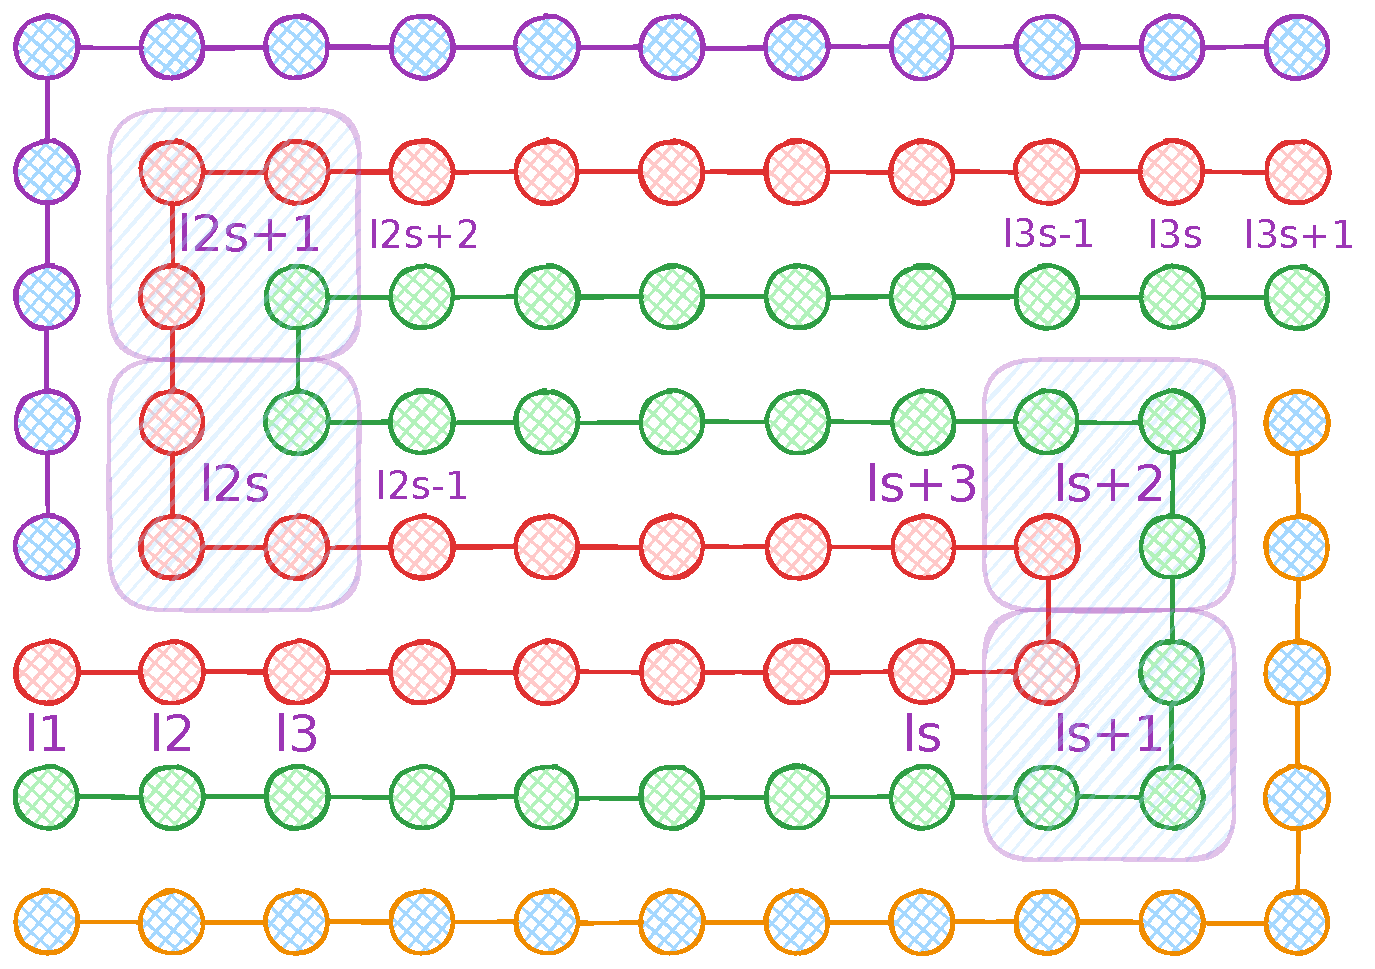
\includegraphics[width=0.7\textwidth]{Chapter3/snake-embedding-simplified.pdf}
        \caption{Snake Embedding technique between the folding dimension and the new dimension}
        \label{fig:chap-3:snake-embedding-visualisation-basic}
    \end{figure}

    \begin{figure}[h!]
        \centering
        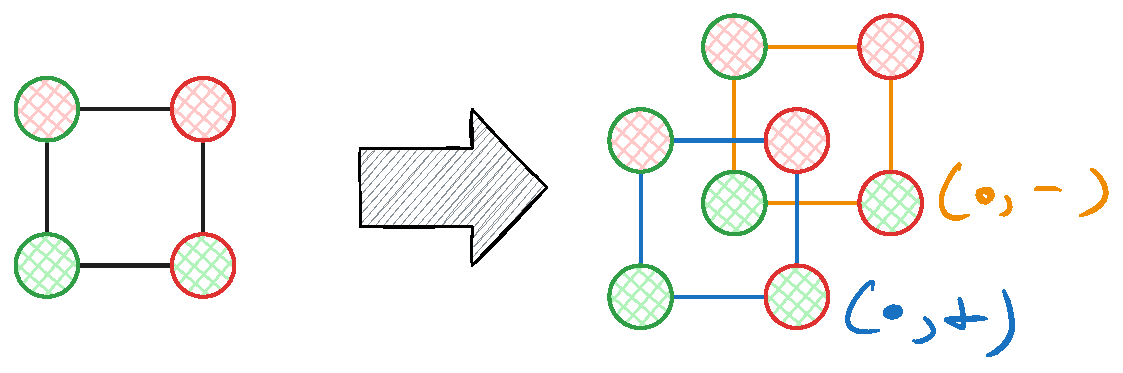
\includegraphics[width=0.7\textwidth]{Chapter3/2d-to-3d-snake-sol.pdf}
        \caption{Snake Embedding technique between the folding dimension and the new dimension}
        \label{fig:chap-3:snake-embedding-2d-to-3d-sol}
    \end{figure}

    To define the above more formally, we define sets $B^U,B^L \subseteq M^{t'}_{n+1}$
    which denote the set of boundary indices of the orange and blue lines.
    In addition, we define functions $\ell^P, \ell^N \subseteq M^{t'}_{n+1}$ to denote the points on the greed and red lines
    with functions $\phi^P, \phi^N$  that are maps $phi^i: \ell^i to M^t_n$ that indicate the indexes in the original space.
    Given our new circuit $\Lambda^{t+1}$, we define the following:
    $$
        \forall x \in M^{t+1}_{n+1}, j\in [n]:  [\Lambda^{t+1}(x)]_j = \begin{cases}
            -1                           & \text{if  }  x \in B^U \cup B^O \wedge x_j > 0 \\
            +1                           & \text{if  }  x \in B^U \cup B^O \wedge x_j = 0 \\
            [\Lambda^{t+1}(\phi^P(x))]_j & \text{if } x \in \ell^P                        \\
            [\Lambda^{t+1}(\phi^N(x))]_j & \text{if } x \in \ell^N                        \\
        \end{cases}
    $$
    For the new dimension, we apply the labelling rules as described previously
    $$
        \forall x \in M^{t+1}_{n+1}:  [\Lambda^{t+1}(x)]_{n+1} = \begin{cases}
            -1 & \text{if  }  x \in B^U \cup \ell^N \\
            +1 & \text{if  }  x \in B^L \cup \ell^P \\
        \end{cases}
    $$
    Using the above we formally define the operation the snake embedding operation $S(T, i)$.

    \begin{definitionbox}{Snake Embedding operation $S(\Lambda^t, i)$}{snake-emb-op}
        Given labelling function $\Lambda: M^t_n \to \{-1, +1\}^n$, apply the snake embedding operation
        on dimension $i \in [n]$, where $m_i \equiv 1 \mod 3$, to a get a new labelling function
        $\Lambda': M'_{n+1} \to \{-1, +1\}^{n+1}$ such that $m'_i = s + 3$, where $\Lambda'$ is defined
        based on the above description.
    \end{definitionbox}

    \begin{claimbox}{Antipodality Solution preservation}{snake-emb-sol-anti}
        Given $\Lambda^t$ which is antipodal, we argue that $\Lambda^{t+1}$
        will remain antipodal.
    \end{claimbox}

    \begin{proof}
        We will prove this by induction. We start with a base case of $2 \to 3$
        and we can observe that all \textit{2D-StrongEoL} instances preserve the antipodality condition.
        Assume we apply snake embedding to one of the two dimensions such that we have $2^n \times y \times z$.
        We can observe that all solutions in the embedded space will be anchored between the red or green lines
        (using figure
        \ref{fig:chap-3:snake-embedding-visualisation-basic}), otherwise the third dimension will not be covered.
        Moreover one can observe can never be anchored in any of the turning points since we have a copy of
        the point and therefore $x,y$ dims will not be covered. We define $\bot^n(\cdot)$ as
        $$ %% TODO
            \forall \bar{p} \in [M]: \bot^n(p) \triangleq \begin{cases}
                1^p\bot & \text{if } \bar{p} < M \\
                1^M     & \text{otherwise} < M   \\
            \end{cases}
        $$
        G

    \end{proof}

    % \begin{claimbox}{Snake Embedding Solution Preservation}{snake-emb-sol-pre}
    %     \label{clm:snake-emb-sol-pre}
    %     Given labelling circuits $\Lambda$ and $\Lambda'$ of the transformed operations:
    %     we say that $|S| = |S'|$, where $S,S'$ define the sets of panchromatic anchor points with respect to the two topologies.
    % \end{claimbox}

    % \begin{proof}
    %     First establish that we cannot have solutions that are anchored within the first two or last two points of the folded space
    %     as it will not satisfy the $k+1$ dimension. It suffices
    %     to show that we can create a bijection between the folded dimension and the unfolded one.

    %     $(\leftarrow)$ Suppose that we have a point $z \in M^{t+1}_{n+1}$ such that the sub-cube $\Lambda^t(z)$ forms a panchromatic square.
    %     We can observe that such solutions will not belong in the turning point areas as is anchor of the cube contain a copy of the subdimension
    %     and since .
    %     The only anchor that can satisfy a panchromatic square
    %     is if it falls on a main or secondary body. Assume $g$ is the index of where $\phi^{-1}(y,z)$ lands one of the bodies and $\bar{g}$ the index of the other body.
    %     Then we can observe that
    %     \begin{align}
    %         \forall z \in h(y,z): [\lambda(g,z)]_{k+1} =  -[\lambda(\bar{g},z)]_{k+1}
    %     \end{align}

    %     Therefore that forms a panchromatic square. Assume that it falls on the cubed regions, we can observe that
    %     $$
    %         \forall z \in *, m \in N(y,z): [\lambda(z,m)]_{y} = [\lambda(y, z)]_{y}
    %     $$
    %     Since it it constant, copying the corner does not affect the solutions.

    %     $(\rightarrow)$ To prove the inverse one can use a similar line of reasoning as the above to demonstrate the same
    % \end{proof}






    % [[1753353759-snake-embeddings 2025-08-01 00.56.15.excalidraw]]





    % $$
    %     \forall x \in [7], y \in [m_{y}], z \in *: \phi(x,y, z) \triangleq \begin{cases}
    %         (y, z)               & \text{if } x \in \{ 1,2 \} \wedge y \in [{s}-1]_{0}                \\
    %         (s+1, z)             & \text{if } (x,y) \in \{ (1, \ell_{s}), (1, s +1), (2, s+1, 2,s) \} \\
    %         (s+2, z)             & \text{if } (x,y) \in \{(3, s), (4, s), (3, s+1), (4, s+1)\}        \\
    %         (2s-1, z)            & \text{if } (x,y) \in \{ (3, 1), (3,2), (4, 1), (4,2) \}            \\
    %         (2s, z)              & \text{if } (x,y) \in \{ (5, 1), (5,2), (6, 1), (6,2) \}            \\
    %         (2s +1 + (y -4) , z) & \text{if } x \in \{ 5,6 \} \wedge y \in \{ 4,\dots, s+ 2\}         \\
    %         (2s -2 -(y-4) , z)   & \text{if } x \in \{ 3,4 \} \wedge y \in \{ 4,\dots, s-1 \}         \\
    %         (2s +1 + (y -4) , z) & \text{if } x \in \{ 5,6 \} \wedge y \in \{ 4,\dots, s+ 2\}         \\
    %     \end{cases}
    % $$


    % $$
    %     \lambda^{k+1}(x) = \begin{cases}
    %         (+, \omega(x_{-(k+1)}))                       & \text{if } x_{k+1} = 0 \vee y = m_{y+1} \wedge x_{k+1} \in [4]_{0}    \\
    %         (-, \omega(x_{-(k+1)}))                       & \text{if } x_{k+1} = 7 \vee y = 0 \wedge x_{k+1} \in \{ 3,\dots, 7 \} \\
    %         (+, \lambda^{k}(\phi(x_{k+1}, x_{y}, x_{r}))) & \text{otherwise}
    %     \end{cases}
    % $$
    % We now show the following lemmata and how they hold for each folding. We will denote the green lines as the main body and the red lines as the second body.
    % Given a sub-hypercube of lengths one, we define as the *anchor* of the cube the corner with the smallest $\|\cdot\|_{1}$ corner.

    % > [!lemma] Panchromatic Square Locations
    % > Every panchromatic square constructed by the snake embedding is anchored at the one of the two bodies




\end{proof}




% \begin{definitionbox}{\textbf{PPAD}-complete}{hf-strong-sperner}
%     \textbf{Input}: A hazard-free circuit $\lambda: [M]^n \to \{-1, +1\}^n$, where $M \in n^{O(1)}$, that describes a \textit{StrongSperner} labelling,
%     as explained in \ref{def:strong-sperner}. For $p \in M$, we use its unary representation, such that $\bar{p} \in M = p \in \{0,1\}^{\lceil \log_2(M) \rceil}$
%     and $\#1(p) = \bar{p}$.
%     \textbf{Output}: We consider a solution a point $p \in \bigtimes_{i \in [n]} M^1$ if and only if:
%     $\lambda(p) =  \bot^n$. 
% \end{definitionbox}



% \subsection{Attempt correlating parsimoniously PureCircuit with the EndOfLine}

